% This file was created by matlab2tikz.
%
%The latest updates can be retrieved from
%  http://www.mathworks.com/matlabcentral/fileexchange/22022-matlab2tikz-matlab2tikz
%where you can also make suggestions and rate matlab2tikz.
%
\definecolor{mycolor1}{rgb}{0.00000,1.00000,1.00000}%
%
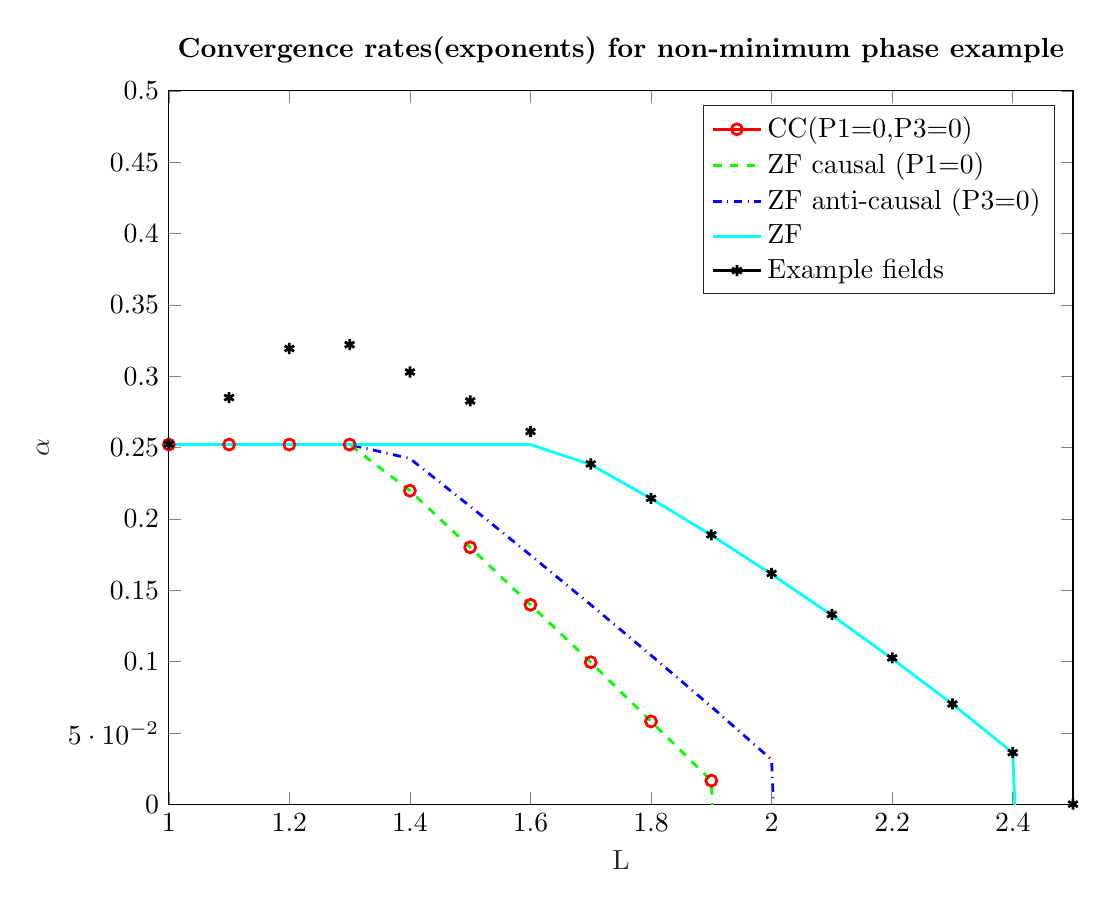
\begin{tikzpicture}

\begin{axis}[%
width=4.521in,
height=3.566in,
at={(0.758in,0.481in)},
scale only axis,
xmin=1,
xmax=2.5,
xlabel style={font=\color{white!15!black}},
xlabel={L},
ymin=0,
ymax=0.5,
ylabel style={font=\color{white!15!black}},
ylabel={$\alpha$},
axis background/.style={fill=white},
title style={font=\bfseries},
title={Convergence rates(exponents) for non-minimum phase example},
legend style={legend cell align=left, align=left, draw=white!15!black}
]
\addplot [color=red, line width=1.0pt, draw=none, mark=o, mark options={solid, red}]
  table[row sep=crcr]{%
1	0.2520751953125\\
1.1	0.2520751953125\\
1.2	0.2520751953125\\
1.3	0.2520751953125\\
1.4	0.2197265625\\
1.5	0.1800537109375\\
1.6	0.1397705078125\\
1.7	0.0994873046875\\
1.8	0.0579833984375\\
1.9	0.0164794921875\\
2	-1\\
2.1	-1\\
2.2	-1\\
2.3	-1\\
2.4	-1\\
2.5	-1\\
2.6	-1\\
2.7	-1\\
2.8	-1\\
2.9	-1\\
3	-1\\
};
\addlegendentry{CC(P1=0,P3=0)}

\addplot [color=green, dashed, line width=1.0pt]
  table[row sep=crcr]{%
1	0.2520751953125\\
1.1	0.2520751953125\\
1.2	0.2520751953125\\
1.3	0.2520751953125\\
1.4	0.2197265625\\
1.5	0.1800537109375\\
1.6	0.1397705078125\\
1.7	0.0994873046875\\
1.8	0.0579833984375\\
1.9	0.0164794921875\\
2	-1\\
2.1	-1\\
2.2	-1\\
2.3	-1\\
2.4	-1\\
2.5	-1\\
2.6	-1\\
2.7	-1\\
2.8	-1\\
2.9	-1\\
3	-1\\
};
\addlegendentry{ZF causal (P1=0)}

\addplot [color=blue, dashdotted, line width=1.0pt]
  table[row sep=crcr]{%
1	0.2520751953125\\
1.1	0.2520751953125\\
1.2	0.2520751953125\\
1.3	0.2520751953125\\
1.4	0.2423095703125\\
1.5	0.208740234375\\
1.6	0.174560546875\\
1.7	0.1397705078125\\
1.8	0.1043701171875\\
1.9	0.068359375\\
2	0.0311279296875\\
2.1	-1\\
2.2	-1\\
2.3	-1\\
2.4	-1\\
2.5	-1\\
2.6	-1\\
2.7	-1\\
2.8	-1\\
2.9	-1\\
3	-1\\
};
\addlegendentry{ZF anti-causal (P3=0)}

\addplot [color=mycolor1, line width=1.0pt]
  table[row sep=crcr]{%
1	0.2520751953125\\
1.1	0.2520751953125\\
1.2	0.2520751953125\\
1.3	0.2520751953125\\
1.4	0.2520751953125\\
1.5	0.2520751953125\\
1.6	0.2520751953125\\
1.7	0.238037109375\\
1.8	0.2142333984375\\
1.9	0.1885986328125\\
2	0.1611328125\\
2.1	0.1324462890625\\
2.2	0.1019287109375\\
2.3	0.0701904296875\\
2.4	0.0360107421875\\
2.5	-1\\
2.6	-1\\
2.7	-1\\
2.8	-1\\
2.9	-1\\
3	-1\\
};
\addlegendentry{ZF}

\addplot [color=black, line width=1.0pt, draw=none, mark=asterisk, mark options={solid, black}]
  table[row sep=crcr]{%
1	0.252381023686084\\
1.1	0.285030034676752\\
1.2	0.319444587967699\\
1.3	0.322120595821607\\
1.4	0.30294136645159\\
1.5	0.282662461122388\\
1.6	0.261201184778797\\
1.7	0.238470096600161\\
1.8	0.214377762177947\\
1.9	0.188829987346274\\
2	0.161731674331652\\
2.1	0.132989449419385\\
2.2	0.102515199007407\\
2.3	0.0702306031940527\\
2.4	0.0360726564236493\\
2.5	-1.11022302462516e-16\\
2.6	-0.0380003387049316\\
2.7	-0.0779064749243448\\
2.8	-0.119656383851905\\
2.9	-0.163144853458106\\
3	-0.208223620537594\\
};
\addlegendentry{Example fields}

\end{axis}
\end{tikzpicture}%